\chapter{系统主要功能设计与实现}

\section{开发及运行环境}
\begin{enumerate}
	\item[(1)] 项目开发环境:
		\begin{itemize}
			\item CPU 最低Intel Core i5 4590或同等性能芯片。
			\item 推荐 Intel Core i7 7700或AMD同等性能芯片及以上。
			\item 内存 最低8GB(推荐16GB及以上)。
			\item 硬盘 需要10GB以上的可用空间(固态硬盘为宜)。
			\item 网络 接入互联网下行20Mbps及以上,上行10Mbps及以上。
			\item 操作系统 macOS Big Sur Version 11.3.1。
			\item 基本软件 JDK-11、MariaDB、Redis、ElasticSearch和Maven。
		\end{itemize}
	\item[(2)] 软件部署环境:
		\begin{itemize}
			\item CPU 最低Intel Core i5 4590或同等性能芯片。
			\item 推荐 Intel Core i7 7700 或AMD同等性能芯片及以上。
			\item 内存 最低8GB(推荐16GB及以上。
			\item 硬盘 需要10GB以上的可用空间(固态硬盘为宜)。
			\item 网络 接入互联网下行20Mbps及以上,上行10Mbps及以上。
		\end{itemize}
\end{enumerate}

\section{系统架构设计}
系统采用B/S(Browser/Server,浏览器/服务器)方式的网络结构,统一采用如Chrome一类的浏览器,通过访问前端服务器获取页面,
前端服务器通过Json向业务服务器发送请求,由Nginx负载均衡分发给各个业务服务器,业务服务器对请求处理后,将结果返回给客户端。
架构设计如图\ref{figure:jiagou}所示。
\begin{figure}[!htbp]
\centering
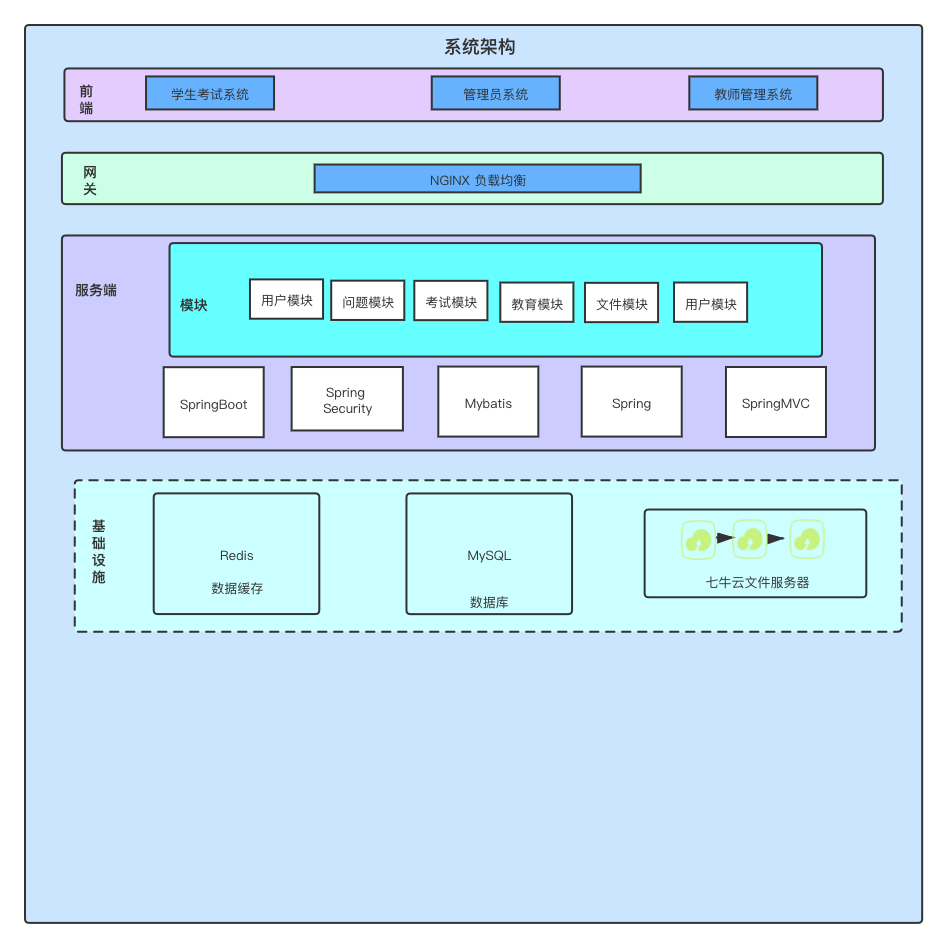
\includegraphics[width=0.6\textwidth,keepaspectratio]{data/chapter-2/jiagou.png}
\caption{系统架构}
\label{figure:jiagou}
\end{figure}

\section{系统各个功能模块的分析与设计}

\subsection{}